\documentclass[11pt,twocolumn]{MyTightStyle}
\usepackage{graphics}
\usepackage{url}
\usepackage{algorithm}
\usepackage{color}
\usepackage{algorithmic}

\markboth{Draft - Do not redistribute}{Draft - Do not redistribute}
\newcommand{\fixme}[1]{{\color{red} #1}}
\newcommand{\comm}[2]{{\color{blue} (#1's comment: #2)}}
\newcommand{\eat}[1]{}

\begin{document}

\title{Churn as a Friend of P2P Overlays, or\\
Playing Shell Games with P2P Identities, or\\
How I Learned to Stop Worrying and Love Churn}

\author{
Tyson Condie\\
\small{UC Berkeley, Berkeley, {CA}}
\and
Varun Kacholia\\
\small{UC Berkeley, Berkeley, {CA}}
\and
Sriram Sankararaman\\
\small{UC Berkeley, Berkeley, {CA}}
\and
Petros Maniatis\\
\small{Intel Research, Berkeley, {CA}}
}

\maketitle

\begin{abstract}
The state of the art of secure routing in peer-to-peer overlays relies
on the certified distribution and rationing of identifiers from a
central, trusted entity.  In this paper, we seek to probe the trade-offs
available when reducing --- or eliminating --- the responsibility of such
a trusted entity.  We propose the use of induced but unpredictable
identifier churn, coupled with routing table diversity in IP network
representation, as a step in that direction, reducing the central,
trusted task to that of a non-interactive emmitter of random nonces.  We
show (very) preliminary evidence that induced churn may provide greater
resistance against malicious peers with many false identities at a
moderate cost in latency and lookup consistency.
\end{abstract}


\section{Introduction}
\label{sec:introduction}
Peer-to-peer overlays, especially when deployed across administrative
domains without an established trust infrastructure, are wide open to
security problems.  Douceur~\cite{Douceur2002short}, Sit and
Morris~\cite{Sit2002short}, and Wallach~\cite{Wallach2002short} survey
important problems that result when malicious peers, especially under
false, ``Sybil'' identities, misbehave to act selfishly, disrupt system services,
or --- worse --- control system services to their advantage.  
Recently, Singh et al.~\cite{Singh2004short} formalized the dirty little
secret of p2p research: a pattern of misbehavior called an \emph{Eclipse
attack}, which consists of the gradual poisoning of good peers' routing
tables with links to a conspiracy of adversarial peers; left unchecked,
the adversary eventually controls most communication between good
peers, thereby placing a stranglehold on the quality and fate of 
services over the overlay.

Current state of the art defenses against Sybil~\cite{Castro2002short}
and Eclipse~\cite{Singh2004short} attacks rely on
centralized components, most notably an authority for the certification
of node identifiers, which eliminates the zero-cost creation of Sybil
identities, and regulates their distribution within the identifier
space~\cite{Castro2002short}.
Though costlier than a completely insecure system, this approach offers
the relief of an existence proof that secure routing in p2p environments
\emph{can} be done.  Especially in environments in which the
administrative and organizational burden of running a
new, central, globally trusted certification authority
is feasible, feasibility of a solid solution is now within grasp.

However, not all environments admit central, unique, globally trusted
certification authorities~\cite{Davis1996short}, for reasons that may
range from lack of trust, to the difficulty of auditing, to low budgets.
In this paper, we explore the design space of possible solutions that
limit required global trust to little more than the trusted components
imposed on end systems by the Internet today: core routers and the
ICANN. Specifically, we investigate three techniques to mitigate the
effects of Sybil and Eclipse attacks: \emph{induced churn},
\emph{synchronized identifier unpredictability}, and \emph{diversity
enforcement}.

Induced churn enforces an upper bound on the lifetime of a peer's
identifier; correct peers observe this lifetime limitation both for
their routing table entries, evicting neighbors with overripe
identifiers, and for their own identifier, changing and moving to a
different logical position in the network regularly.

Synchronized identifier unpredictability expands on the common technique
of limiting the choice of a peer's identifiers to a few deterministic
transformations of that peer's IP address.  Our extension requires that
the appropriate transformation from a peer's IP address to its network
identifier be unknown and unpredictable until that peer is ready to
start using that identifier.  In conjunction with induced churn, this
means that a peer does not know where it will be in the logical
structure of the network until it is time to move there.

Diversity enforcement ensures that identities on which a peer relies for
correct operation (e.g., in a peer's routing table)
are hard to spoof by the same faulty entity.  For example, by enforcing
that no two
entries in the same routing table correspond to IP addresses within the
same subnet, a correct peer can mitigate the effect of a single
malicious entity's zero-cost
spoofing capabilities.

The objective of these three techniques is to hinder all three phases of
a Sybil and Eclipse attacker's battle plan (in fact, of any battle
plan): strategy, tactics, and entrenchment.  Strategy of node placement
in the network to cause maximum damage against the network itself or
particular peers is reduced to short-term projections only, since no-one
knows, including the adversary, what the network will look like after
all current identifiers have had to change unpredictably.  Tactics, or
``how to get there'' once a strategy has been formed, is hindered by
diversity enforcement, which drastically reduces the number of possible
IP addresses that an adversary can claim (via spoofing); for a given
adversarial network foothold, this effectively acts as a rate limiter of
improvements on the adversary's position in correct peers' routing
tables.  Entrenchment, or ``how to stay there,'' is directly undermined
by induced churn, which makes transient any ``strategically desirable''
positions the adversary has acquired.

We describe a strawman design for a p2p system that incorporates all of
the above techniques, exploring the trade-offs inherent in the design
choices for each technique.  We also present evidence from a preliminary
evaluation on Bamboo~\cite{Rhea2004short}, a
fine-tuned, real DHT, that our techniques are a promising research
direction towards eliminating or severely reducing the need for
centralized components  in the war against Sybil and Eclipse
attacks.
With this preliminary investigation, we hope to
resuscitate a discussion of p2p security that does not presuppose
centralized certification authorities beyond those that we already
tolerate on the Internet today.


\section{Defenses}
\label{sec:defenses}

In this section, we begin by presenting our system model and then
describe our three
defenses. For each defense, we outline our design as well as some
alternatives, some of which we plan to evaluate further. 

In our system model, router malice is concentrated on the edges of the
Internet. This means that a good peer performing successfully a 3-way IP
handshake with a destination knows that it is contacting a destination
within ``eavesdropping distance'' of the intended destination
(typically, within the same IP subnet) or a local eavesdropper.  We
assume that a single malicious entity can only spoof IP addresses within
its subnet, and that the largest such ``spoofable'' subnet is a /24
(i.e., contains 254 possible addresses).  We call the top 3 bytes of an
IP address its \emph{unspoofable identifier}.

The adversary has instantaneous control over a fraction of the
peer population, the \emph{malicious peers}.  For the purposes
of this paper, all peers sharing an unspoofable identifier with a
malign peer are considered malicious.


\subsection{Synchronized Identifier Unpredictability}
\label{sec:unpredictability}

In many p2p overlays, a peer's identifier is cryptographically derived
from its IP address (e.g., $\mathit{nodeID} =
\mathrm{SHA1}(\mathit{NodeIP})$) to ensure a uniform distribution of
identifiers and
to mitigate the strategic choice of identifiers by malicious peers.

In our approach, this mapping from an IP address to an identifier also
includes a random nonce that is unpredictable and unbiasable by the peer
identified (i.e., $\mathit{nodeID} = \mathrm{SHA1}(\mathit{random} \|
\mathit{NodeIP})$).  To obtain this random number, we use a centralized,
trusted, unpredictable logical clock, the \emph{randomness oracle}.  It
produces timed random numbers as \{Time, Random Number\} signed
statements, at a coarse time granularity (e.g., every 10 seconds per
time-step).  

Our design choice places the responsibility of keeping time and producing
unpredictability to a centralized oracle.  This is a reduction in
central responsibility, compared to the alternative of having a
certification authority registering entities, controlling the rate at
which identifiers are issued, dealing with revocation, etc.  An
intermediate design point between the two would be to control
identifier unpredictability over entire groups of peers (according to some
groupping), reducing the
state maintained at the server from the granularity of individual
addresses to that of groups, but moving the burden of address-to-group
assignment and enforcement, from the server to the peers themselves.

Going in the opposite direction from our design choice towards less
centralized responsibility, we could distribute the task of controlling
unpredictability, for instance by using variants of shared coin flipping
schemes, such as that described by Cachin et al.~\cite{Cachin2000short}.
The randomness oracle could thus be distributed over all peers or a set
of servers enjoying partial trust among the peer population.  This, for
instance, could be a task for the set of bootstrapping servers that most
p2p overlays rely on.

Finally, an attractive, entirely self-centered design we are considering
for future work would help an individual peer to ensure that identifiers
of peers it communicates with are determined in a manner unpredictable
to them and fresh within a time frame that the peer itself can track
alone.  The basic idea is to run an unpredictable logical clock per
peer.  At every time-step, each peer broadcasts the random value of its
clock to its neighbors.  A peer receiving clock values from its
neighbors hashes them together (e.g., in a Merkle hash tree) and
combines the result with its own previous clock value to produce a value
at the next time-step.  A peer's identity is cryptographically dependent
on the value of its local logical clock.

To prove to a neighbor that its identifier is relatively fresh and until
recently unpredictable, a peer traces a backward path from the clock
value that influenced its new identifier to a clock value issued by this
new neighbor some time in the past; this path follows backwards a
sequence of hashes and logical clock value broadcasts, e.g., tracing a
path from the new neighbor to the peer's old position in the overlay.
Since the neighbor remembers when it issued its own clock values (for a
short period in the past), it can estimate for how long the peer has
known its new identifier.  This is a simplified instance of the
coordination required for a distributed secure time stamping
service~\cite{Maniatis2002bshort}.  We are planning to explore the
overheads and potential benefits of such an aggressively decentralized
approach under heavy churn.


\subsection{Induced Churn}
\label{sec:churn}

Peers enforce a cap on the maximum length of an identity lifetime.
To control this effectively at the time granularity imposed by the
randomness oracle, we organize peers into $G$ \emph{churn groups}.  Peers in the same
group churn their identities at the same time-step of the randomness oracle.
Each identity has a fixed maximum lifetime of $T = k \times G$
time-steps, where $k$ is a positive constant ($k = 1$ in our
current design).   
Identifier changes of churn groups over time are staggered to occur at a rate
of one group-wide identifier change every $k$ time-steps.  As a result, in
$T$ time-steps, all peers in all groups have churned identifiers once.

Peers pick a churn group according
to their unspoofable identifier, i.e., the top $u$ bits of their IP
address --- we set $u=3$ here --- e.g., by cryptographically hashing the
unspoofable identifier
mod $G$.  A group is mapped to the time-step at which it must churn
using a straightforward wrap-around mapping, i.e., group $g$ churns at all
time-steps $e$ such that $e/T = g\ \mathrm{mod}\ G$.

A new identity is unpredictable until the associated random number has
been emmitted by the server.  Everyone knows
an entity's identity for the current and several prior changes.

A peer has some time to prepare for an identity change, after it finds
out what its next identifier is going to be.  It uses that time to
construct a first version of its future routing table with its new
identifier which we call the \emph{prospective routing table}.  For that purpose, peers maintain a \emph{constrained
routing table} in the manner described by Castro et
al.~\cite{Castro2002short}; this table limits the possible choices for
each routing table entry, thereby being less amenable to tampering. When
a peer's current idenfier expires, it switches to its precomputed
routing table for the next identifier.


We considered several alternative ways for inducing churn in the system, including
proximity metric randomization, gang evictions, and selfish routing
table churning.  Proximity metric randomization introduces error in the
measurement of the proximity metric used for routing optimization.  For the
example of point-to-point latency as the metric, we could randomize
several low-order bits of the measured latency per discovered peer.
Though coarse-grained differentiation among potential links
is still available, finer-grained comparisons of links change
unpredictably, causing proximity neighbor selection not to
converge always to the strictly closest neighbor  but, instead, to pick
at random from a larger set of otherwise nearby neighbors.  This
approach seemed awkward.

Gang evictions would allow the peers currently occupying a neighborhood
of the logical overlay space collectively to decide the order of peer
evictions and to monitor joins.

Selfish routing-table churning follows the similar philosophy of evicting entries
from a peer's routing table when those entries have exceeded a maximum
lifetime.  However, an identifier is not evicted from all routing tables
of correct peers at the same time.  As a result, though similar, this
technique might lead to a continuous state of routing
inconsistencies~\cite{Liben2002short}.





\subsection{Diversity Enforcement}

Peers cap the maximum number of identities within routing tables and
leaf sets that are likely to be owned by the same entity, potentially a
spoofer.  The better our estimator of such identities, the harder an
adversary must try to place many of his identities into a correct peer's
routing tables and leaf sets.  Our design limits the number of entries
in a peer's routing table and leaf set that may share unspoofable
identifiers (i.e., subnets).

Although our design choice  does not impede an adversary who
controls multiple entities in distinct IP networks, it increases 
the cost of this behavior pattern beyond the means of a lonely spoofer.
Furthermore, this technique facilitates the productive use of induced
churn, since it prevents a malicious peer recently churned out of a
routing table from coming right back in under a different identifier
from a ``nearby'' address.

Alternatively, others have proposed client puzzles as an enforcer of
``entity diversity.''  In that fashion, an adversary with constrained
physical resources (e.g., computation, network bandwidth, memory,
storage) can only masquerade as a finite number of identities.  Douceur
suggest that such approaches alone may not work without
centralization~\cite{Douceur2002short}.




\section{Architecture}
\label{arch} 
We propose a distributed collaborative scheme that existing domain mail servers can use along with other techniques (conventional blacklists and content-based filtering schemes), for detecting spam. Figure~\ref{fig:architecture} provides a high level overview of the architecture along with the overlay network topology that is used for sharing information. The architecture diagram shows a logical separation between super-nodes that are connected in a peer-to-peer fashion to aggregate information for clustering. The super-nodes form the backend of the system. We can have settings where domain mail servers or nodes at an enterprise having relationship with the domains, can act as super nodes. The peer-to-peer network of super-nodes forms the backend of our system. These nodes aggregate the information about the traffic of spammers and perform clustering. The cluster information is sent back to the domain mail servers. Classification of new received emails is performed locally at the domain mail servers.

Currently we have implemented the backend of the system that has a set of super-nodes running the clustering algorithm in a distributed fashion. In section~\ref{future} we discuss further work that will make the system scalable and deployable in the real-world. Section~\ref{arch-cluster} explains the backend architecture and gives details on how clustering is performed in the system. In section~\ref{arch-classify} we explain how the domain mail servers can use the cluster information to detect spammers. The distributed implementation of the backend is discussed in section~\ref{sec:distP2}.

\begin{figure}[t]%{4.25in}
\centering
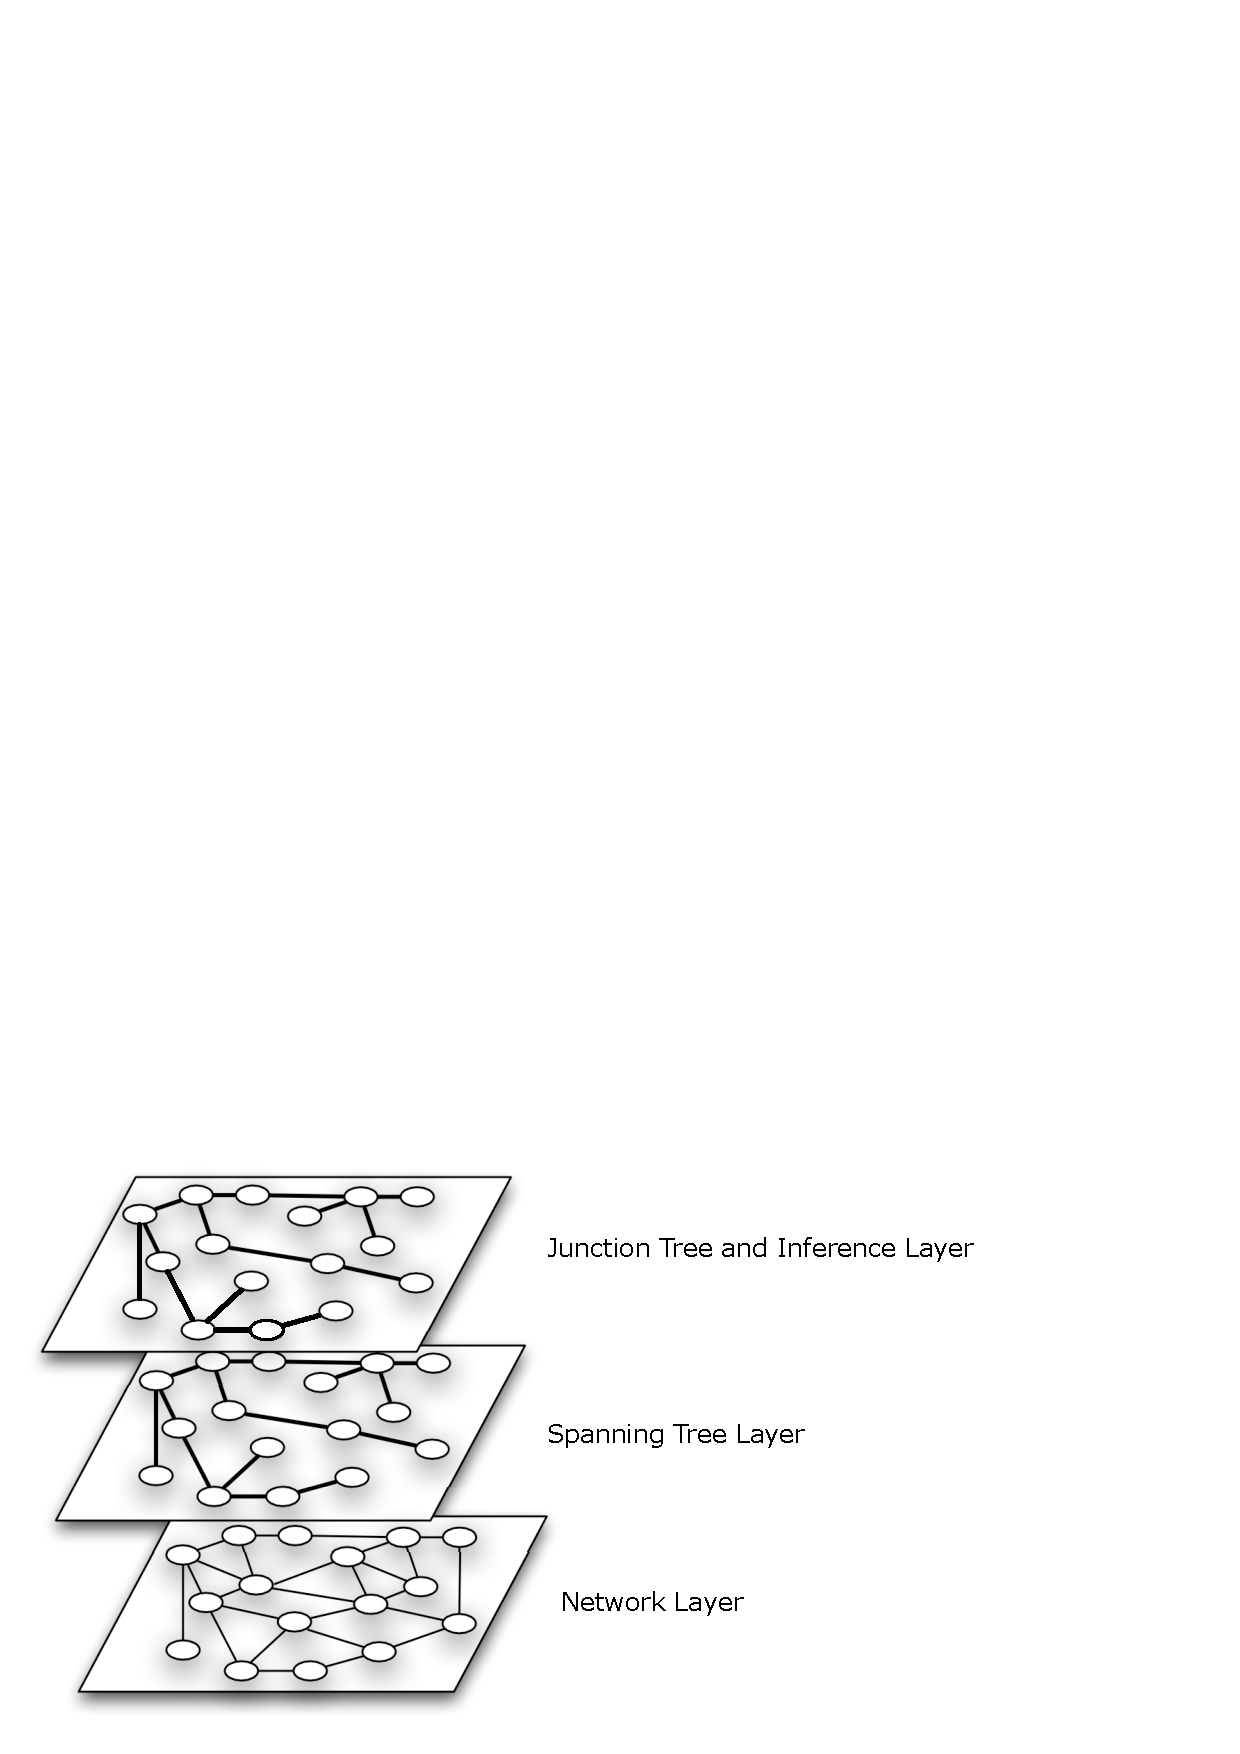
\includegraphics[width=0.45\textwidth]{figures/architecture.pdf}
\caption{High level overview of the architecture. The compression block is not implemented currently}
\label{fig:architecture}
\end{figure}
\subsection{Clustering}
\label{arch-cluster}

Affinity propagation calculates clusters that are refined iteratively by performing clustering over the information periodically collected from domain mail servers. This information for clustering includes details regarding the frequency of emails a domain rejects from spammers. This can be obtained from domain mail servers that use conventional filters to filter spam~\cite{spamassassin} . The list can also be enriched from user feedback on spam emails as well. We use the dataset that \emph{SpamTracker} \cite{bb} used for clustering, which contains the information regarding the frequency of emails from spammers that a domain receives. The dataset is from an email hosting provider's decisions about early mail rejects from hundreds of domains. More details about the data can be found in section~\ref{sec:data}. 

The spammer's activity at a particular domain is sent to a super-node that is geographically close to the domain mail server. Chord is used to lookup the super-node that corresponds to the location where the data of the IP address is aggregated. The super-nodes aggregate the IP address activity across all domains. The aggregated information for each IP address represents the row in matrix $M$ (Equation~\ref{eq:collapse}) for the IP address.  Section~\ref{future} discusses details on how aggregation can be accomplished with domain mail servers acting as super-nodes connected in a peer-to-peer network in a scalable fashion. 

After the aggregation has been performed, similarity of an IP address's sending pattern with other IP address is calculated (Equation~\ref{eq:similarity}). This similarity information forms the basis for clustering. The clusters, calculated by running affinity propagation, are sent back to the domain mail servers, communicating the sending patterns of spammers.

The clusters are refined periodically after \emph{$\bigtriangleup t$} time interval. We choose \emph{$\bigtriangleup t$} to be 6 hours (the same value as chosen by Ramachandran \cite{bb}) but this can be made configurable and changed randomly to overcome evasion \footnote{Refer to Section~\ref{future} for further discussion on evasion}. Email rejection information for \emph{$t+\bigtriangleup t$} is collected and sent to the super-nodes for updating the clusters.
\subsection{Classification}
\label{arch-classify}

Whenever a domain mail server receives an email it creates or appends the sending information for the IP address to its own logs. This information is shared with other mail servers after a brief period of time. The server then calculates the score of the IP address' sending pattern with respect to the recent cluster information stored locally. Classification can be performed in real-time and locally. The magnitude of the score \emph{S} computed using Equation~\ref{eq:score} determines how closely the sending pattern of the IP address matches a spammer's sending pattern. Each domain mail server can incorporate its own threshold value for the score and decide actions to be performed against emails that have a higher score than the threshold.

\subsection{P2 Distributed Implementation}
\label{sec:distP2}

Our current work involves implementation of the backend of the system. The backend has a set of super-nodes running the affinity propagation clustering algorithm in a distributed fashion. Affinity propagation is implemented in P2 and is run on all super-nodes. The affinity propagation overlog has three main relations similarity, responsibility and availability. The similarity relation stores the similarity each local IP address has with other IP addresses. Responsibilities and availabilities are initialized to zero and updated at regular time intervals equal to AP\_EPOCH. Relation sentResponsibility is used to store the responsibilities sent by a node. This information saves us from doing a round-trip while calculating the exemplars. Refer to Appendix~\ref{appendix} to have a look at the detailed overlog. For brevity, we have not shown the damping factor calculations, initialization messages and Chord integration for lookup of data location. Materialized table variable stores the location of the IP address. We have modified the algorithm to work for multiple variables per node and the localVariable table stores the information of IP addresses associated with a super-node.

Each super-node stores information regarding the similarity of a set of IP addresses. The similarity is calculated using Equation~\ref{eq:similarity}. 
These super-nodes send messages, locally or to remote nodes that have IP addresses with similar sending behavior to the local IP addresses.

To reduce the amount of information aggregated at the super-nodes, we took a greedy approach for performing \emph{cluster compression}. This approach reduces the number of IP addresses that have to be clustered and thus reduces the computation performed for clustering. Each row in the complete matrix $M$ (Equation~\ref{eq:collapse}) is classified with the cluster averages. Rows having high scores (Equation~\ref{eq:score}) are removed from the matrix and their sending information is incorporated into the previous clusters. This is computed by averaging the new rows and the cluster (Equation~\ref{eq:cavg}) to get the updated clusters. A new matrix is formed, which includes the new clusters along with a mutually exclusive random sample of IP addresses that sent email during this same \emph{$\bigtriangleup t$} interval. This \emph{n}x\emph{d} matrix is used for affinity propagation as before. 

\section{Evaluation models}

Consider the \emph{successor} relation described above.  According to our intuitive interpretation, this relation models
the passage of time, in order to establish a temporal order among ground atoms.  More formally, we expect of a successor
relation $S$ that

$\forall A,B (successor(A, B) \rightarrow B > A) \land \forall A \exists B (successor(A, B))$

This implies that successor is infinite (as we'd expect time to be).  This is problematic because it leads to unsafe programs.

\newtheorem{example}{Example}
\begin{example}
Consider the program and EDB below.

\begin{Dedalus}
r1
p_pos(A, B)@next \(\leftarrow\)
  p_pos(A, B),
  \(\lnot\)p_neg(A, B);
  
p_pos(A, B)  \(\leftarrow\)
  p(A, B);
  
p(1, 2)@123;
  
\end{Dedalus}

The single ground fact will, due to \emph{r1}, cause as many deductions as there are tuples in the successor relation.

\end{example}

But if \emph{successor} is infinite, many of mthese are in some sense \emph{void deductions}, functionally determined based on the EDB.
The EDB determines a window over successor that is relevant to any computation that must be performed.  It is easy
to see that in this example, we need only consider a successor relation that contains a single tuple \{123, 124\}.

Consider the given EDB extended with two more facts:

\begin{Dedalus}
delete p(1, 2)@456;
p(?, ?)@789;
\end{Dedalus}

Evaluating this program and EDB will require a \emph{successor} relation with values that range from 123 - 789.

\begin{definition}
A \emph{post-hoc} evaluation is an evaluation of a Dedalus program in which the EDB is given, \emph{successor} is derived from it
as part of a fixpoint computation.
\end{definition}

In a post-hoc evaluation, we may use the given EDB to populate the successor relation in the following way:

Define first a second order predicate called \emph{event\_time} 
that contains the union of the time attributes from the trace of events. Let \emph{Trace} be the set of $n$ EDB predicates.  
Then \emph{event\_time} is defined as

$event\_time(\Tau) \leftarrow \displaystyle\bigcup_{i}^n \pi_{\Tau}Trace_{i}$

\begin{Dedalus}
smax(max<N>) \(\leftarrow\) event\_time(N);
smin(min<N>) \(\leftarrow\) event\_time(N);

successor(N, N + 1) \(\leftarrow\) smin(N);

successor(S, S + 1) \(\leftarrow\) 
    successor(N, S),
    smax(M),
    N <= M;
\end{Dedalus}

In a post-hoc evaluation, time is in some sense ``instantaneous" in that all values of the successor relation are considered in a single
fixpoint computation.  
\paa{notes follow}


define a trace as a list of events ordered by time.  then the property we want to prove is about prefix computations.  take a function FP that returns an IDB.  We'll use 
the notation $\Gamma$ to indicate a trace, and $\alpha_{1} \ldots \alpha_{n}$ to indicate prefixes of  $Gamma$. $\alpha_{n} = \Gamma$, and since every
$\alpha$ is an increasing subset of the EDB, we have 

$\forall \alpha_{i}, \alpha_{j} \in \Gamma ((i < j) \to (\alpha_{i} \subset \alpha_{j}))$.

We would like to show that 

$FP(\alpha_{k}) =  \displaystyle \bigcup_{i=0}^{k} FP(\alpha_{i})$ for any $k$.  

this could (with some work) lead to an inductive proof
that an infinite model is minimal.


%%   FP(alpha_{k} \union FP(alpha_{k-1} \union

if we have this, then we have:

Any posthoc evaluation is equivalent to any 


\section{Discussion}
\label{sec:futureWork}



Certification authorities.

Towards a trusted random clock.


\section{Conclusion}
We have presented our initial work that explores the potential of three techniques
to defend against Sybil and Eclipse attacks. Limiting the lifetime of a peer's 
location in the overlay network curbs that peer's ability to conduct these 
attacks. Induced churn imposes a sliding window over a peer's location in the 
overlay. Synchronized identifier unpredictability ensures that peers are unable 
to see outside of this sliding window. By enforcing diversity we limit the number
of references a peer is able to inject into the routing state of others. 

Our strawman design to these techniques describes a protocol that enforces 
peers churning at specific times in an unpredictable way. It requires the use of 
a centralized component to distributed timed random numbers as signed
statements. As future work we plan to distribute the responsibility of unpredictability 
to the individual peers through the use of an unpredictable logical clock. Peers would
produce a random number for the next time-step by hashing the values of their
logical clocks.

\eat{
\section{Related Work}
\label{sec:relatedWork}

Peer-to-peer systems are difficult to protect against malicious incursions.  Current work in that direction simplifies the problem in significant ways:  Castro et al introduce a central certification authority, SOS limits the population to system-wide known membership, LOCKSS deals with leisurely changing conditions, EigenTrust ranks peers based on good behavior. A common goal of these systems is to ensure that the fraction of traffic under malicious control is no more than the fraction malicious nodes in the network.

Castro et al.~\cite{Castro2002short} describe an enhancement of the Pastry overlay system~\cite{Rowstron2001short} to deal with malicious activity, including routing table poisoning, message misrouting, and Sibyl attacks.  Singh et al.~\cite{Singh2004short} extend this work to handle \emph{eclipse} attacks in general overlays (structured or unstructured) by limiting the in- and out-degree of the overlay graph. The neighbor limit reduces the number of routing table and leaf set entries a malicious node can occupy, and consequently the level of poisoning. Although very promising, these proposals rely on a centralized authority for the assignment of both node identifiers and public key certificates.  In this work, we seek to pursue the same goal but without requiring such a powerful, trusted, central entity for correctness.  We replace this central entity with the randomness oracle, which is a much simpler and cheaper trusted entity.

Kamvar et al.~\cite{EigenTrust} base the decision of whether to interact with a particular peer on the reputation of that peer. The paper describes a distributed ranking primitive similar to the PageRank algorithm~\cite{pagerank} that does not require the use of a centralized server. Peers avoid interactions  (e.g., file downloads, links to other peers) with other peers that do not have good reputations. Their simulated results show that interactions with malicious peers are avoided under a certain malicious fraction (around 0.2) of the population. The proposed scheme could be incorporated into our model by avoiding routing table or leaf set entries with poor reputation scores. However, what determines a "good" reputation score is not always evident\footnote{The paper simply chooses the peer with the best reputation score.}. Moreover, it remains to be seen whether such a primitive can be trusted to provide accurate reputation scores in an open system.
}

\bibliographystyle{plain}
\bibliography{bibliography}


\end{document}

